% This file was created with matplot2tikz v0.5.3.
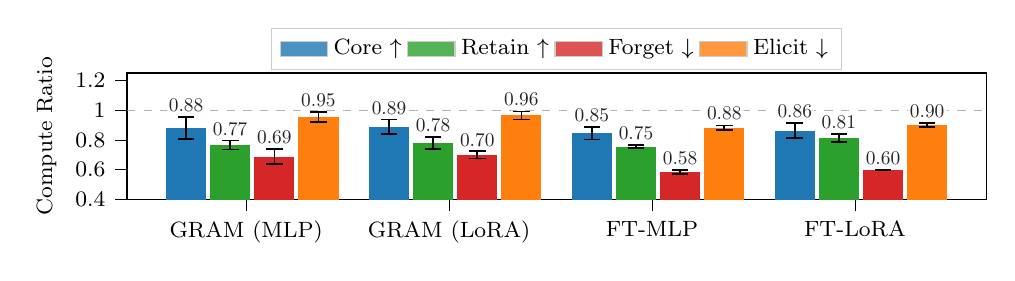
\begin{tikzpicture}

\definecolor{crimson2143940}{RGB}{214,39,40}
\definecolor{darkgray176}{RGB}{176,176,176}
\definecolor{darkorange25512714}{RGB}{255,127,14}
\definecolor{forestgreen4416044}{RGB}{44,160,44}
\definecolor{gray}{RGB}{128,128,128}
\definecolor{lightgray204}{RGB}{204,204,204}
\definecolor{steelblue31119180}{RGB}{31,119,180}

\begin{axis}[
label style={font=\footnotesize},
tick label style={font=\footnotesize},
scale only axis=true,
width=0.9\linewidth,
height=0.13245\linewidth,
legend cell align={left},
legend columns=4,
legend style={
  font=\footnotesize,
  fill opacity=0.8,
  draw opacity=1,
  text opacity=1,
  at={(0.5,1.02)},
  anchor=south,
  draw=lightgray204
},
tick align=outside,
tick pos=left,
x grid style={darkgray176},
xmin=-0.5875, xmax=3.6475,
xtick style={color=black},
xtick={0,1,2,3},
xticklabels={GRAM (MLP),GRAM (LoRA),FT-MLP,FT-LoRA},
y grid style={darkgray176},
ylabel={Compute Ratio},
ymin=0.4, ymax=1.25,
ytick style={color=black}
]
\draw[draw=none,fill=steelblue31119180] (axis cs:-0.395,0) rectangle (axis cs:-0.1975,0.88160841720975);
\addlegendimage{area legend,draw=none,fill=steelblue31119180}
\addlegendentry{Core $\uparrow$}

\draw[draw=none,fill=steelblue31119180] (axis cs:0.605,0) rectangle (axis cs:0.8025,0.888523523543281);
\draw[draw=none,fill=steelblue31119180] (axis cs:1.605,0) rectangle (axis cs:1.8025,0.845571532339865);
\draw[draw=none,fill=steelblue31119180] (axis cs:2.605,0) rectangle (axis cs:2.8025,0.863014712260671);
\draw[draw=none,fill=forestgreen4416044] (axis cs:-0.1775,0) rectangle (axis cs:0.02,0.765736314123483);
\addlegendimage{area legend,draw=none,fill=forestgreen4416044}
\addlegendentry{Retain $\uparrow$}

\draw[draw=none,fill=forestgreen4416044] (axis cs:0.8225,0) rectangle (axis cs:1.02,0.779863270945771);
\draw[draw=none,fill=forestgreen4416044] (axis cs:1.8225,0) rectangle (axis cs:2.02,0.754039425216177);
\draw[draw=none,fill=forestgreen4416044] (axis cs:2.8225,0) rectangle (axis cs:3.02,0.812507144360484);
\draw[draw=none,fill=crimson2143940] (axis cs:0.04,0) rectangle (axis cs:0.2375,0.687713773040091);
\addlegendimage{area legend,draw=none,fill=crimson2143940}
\addlegendentry{Forget $\downarrow$}

\draw[draw=none,fill=crimson2143940] (axis cs:1.04,0) rectangle (axis cs:1.2375,0.699145994029608);
\draw[draw=none,fill=crimson2143940] (axis cs:2.04,0) rectangle (axis cs:2.2375,0.584388029773255);
\draw[draw=none,fill=crimson2143940] (axis cs:3.04,0) rectangle (axis cs:3.2375,0.596357284192256);
\draw[draw=none,fill=darkorange25512714] (axis cs:0.2575,0) rectangle (axis cs:0.455,0.95493882321213);
\addlegendimage{area legend,draw=none,fill=darkorange25512714}
\addlegendentry{Elicit $\downarrow$}

\draw[draw=none,fill=darkorange25512714] (axis cs:1.2575,0) rectangle (axis cs:1.455,0.964356298153923);
\draw[draw=none,fill=darkorange25512714] (axis cs:2.2575,0) rectangle (axis cs:2.455,0.882449345244797);
\draw[draw=none,fill=darkorange25512714] (axis cs:3.2575,0) rectangle (axis cs:3.455,0.901772014944681);
\path [draw=black, semithick]
(axis cs:-0.29625,0.808289964278567)
--(axis cs:-0.29625,0.954926870140933);

\path [draw=black, semithick]
(axis cs:0.70375,0.838956718782511)
--(axis cs:0.70375,0.938090328304051);

\path [draw=black, semithick]
(axis cs:1.70375,0.802764742471458)
--(axis cs:1.70375,0.888378322208273);

\path [draw=black, semithick]
(axis cs:2.70375,0.811675803611189)
--(axis cs:2.70375,0.914353620910153);

\addplot [semithick, steelblue31119180, mark=-, mark size=3, mark options={solid,draw=black}, only marks]
table {%
-0.29625 0.808289964278567
0.70375 0.838956718782511
1.70375 0.802764742471458
2.70375 0.811675803611189
};
\addplot [semithick, steelblue31119180, mark=-, mark size=3, mark options={solid,draw=black}, only marks]
table {%
-0.29625 0.954926870140933
0.70375 0.938090328304051
1.70375 0.888378322208273
2.70375 0.914353620910153
};
\path [draw=black, semithick]
(axis cs:-0.07875,0.735883974437814)
--(axis cs:-0.07875,0.795588653809151);

\path [draw=black, semithick]
(axis cs:0.92125,0.73991415070663)
--(axis cs:0.92125,0.819812391184911);

\path [draw=black, semithick]
(axis cs:1.92125,0.744040058681754)
--(axis cs:1.92125,0.764038791750599);

\path [draw=black, semithick]
(axis cs:2.92125,0.784381869270275)
--(axis cs:2.92125,0.840632419450693);

\addplot [semithick, steelblue31119180, mark=-, mark size=3, mark options={solid,draw=black}, only marks]
table {%
-0.07875 0.735883974437814
0.92125 0.73991415070663
1.92125 0.744040058681754
2.92125 0.784381869270275
};
\addplot [semithick, steelblue31119180, mark=-, mark size=3, mark options={solid,draw=black}, only marks]
table {%
-0.07875 0.795588653809151
0.92125 0.819812391184911
1.92125 0.764038791750599
2.92125 0.840632419450693
};
\path [draw=black, semithick]
(axis cs:0.13875,0.637949563822205)
--(axis cs:0.13875,0.737477982257976);

\path [draw=black, semithick]
(axis cs:1.13875,0.674697633959033)
--(axis cs:1.13875,0.723594354100182);

\path [draw=black, semithick]
(axis cs:2.13875,0.572886251182923)
--(axis cs:2.13875,0.595889808363586);

\path [draw=black, semithick]
(axis cs:3.13875,0.594065128356306)
--(axis cs:3.13875,0.598649440028207);

\addplot [semithick, steelblue31119180, mark=-, mark size=3, mark options={solid,draw=black}, only marks]
table {%
0.13875 0.637949563822205
1.13875 0.674697633959033
2.13875 0.572886251182923
3.13875 0.594065128356306
};
\addplot [semithick, steelblue31119180, mark=-, mark size=3, mark options={solid,draw=black}, only marks]
table {%
0.13875 0.737477982257976
1.13875 0.723594354100182
2.13875 0.595889808363586
3.13875 0.598649440028207
};
\path [draw=black, semithick]
(axis cs:0.35625,0.920274864604228)
--(axis cs:0.35625,0.989602781820032);

\path [draw=black, semithick]
(axis cs:1.35625,0.936888455919162)
--(axis cs:1.35625,0.991824140388684);

\path [draw=black, semithick]
(axis cs:2.35625,0.867646303111356)
--(axis cs:2.35625,0.897252387378238);

\path [draw=black, semithick]
(axis cs:3.35625,0.889010793653403)
--(axis cs:3.35625,0.914533236235958);

\addplot [semithick, steelblue31119180, mark=-, mark size=3, mark options={solid,draw=black}, only marks]
table {%
0.35625 0.920274864604228
1.35625 0.936888455919162
2.35625 0.867646303111356
3.35625 0.889010793653403
};
\addplot [semithick, steelblue31119180, mark=-, mark size=3, mark options={solid,draw=black}, only marks]
table {%
0.35625 0.989602781820032
1.35625 0.991824140388684
2.35625 0.897252387378238
3.35625 0.914533236235958
};
\addplot [line width=0.28pt, gray, opacity=0.6, dashed, forget plot]
table {%
-0.5875 1
3.6475 1
};
\draw (axis cs:-0.29625,0.973537081358786) node[
  scale=0.7,
  fill=white,
  draw=none,
  line width=0.4pt,
  inner sep=1.1pt,
  fill opacity=0.85,
  anchor=south,
  text=black,
  rotate=0.0
]{0.88};
\draw (axis cs:0.70375,0.956700539521903) node[
  scale=0.7,
  fill=white,
  draw=none,
  line width=0.4pt,
  inner sep=1.1pt,
  fill opacity=0.85,
  anchor=south,
  text=black,
  rotate=0.0
]{0.89};
\draw (axis cs:1.70375,0.906988533426126) node[
  scale=0.7,
  fill=white,
  draw=none,
  line width=0.4pt,
  inner sep=1.1pt,
  fill opacity=0.85,
  anchor=south,
  text=black,
  rotate=0.0
]{0.85};
\draw (axis cs:2.70375,0.932963832128005) node[
  scale=0.7,
  fill=white,
  draw=none,
  line width=0.4pt,
  inner sep=1.1pt,
  fill opacity=0.85,
  anchor=south,
  text=black,
  rotate=0.0
]{0.86};
\draw (axis cs:-0.07875,0.814198865027003) node[
  scale=0.7,
  fill=white,
  draw=none,
  line width=0.4pt,
  inner sep=1.1pt,
  fill opacity=0.85,
  anchor=south,
  text=black,
  rotate=0.0
]{0.77};
\draw (axis cs:0.92125,0.838422602402763) node[
  scale=0.7,
  fill=white,
  draw=none,
  line width=0.4pt,
  inner sep=1.1pt,
  fill opacity=0.85,
  anchor=south,
  text=black,
  rotate=0.0
]{0.78};
\draw (axis cs:1.92125,0.782649002968451) node[
  scale=0.7,
  fill=white,
  draw=none,
  line width=0.4pt,
  inner sep=1.1pt,
  fill opacity=0.85,
  anchor=south,
  text=black,
  rotate=0.0
]{0.75};
\draw (axis cs:2.92125,0.859242630668546) node[
  scale=0.7,
  fill=white,
  draw=none,
  line width=0.4pt,
  inner sep=1.1pt,
  fill opacity=0.85,
  anchor=south,
  text=black,
  rotate=0.0
]{0.81};
\draw (axis cs:0.13875,0.756088193475828) node[
  scale=0.7,
  fill=white,
  draw=none,
  line width=0.4pt,
  inner sep=1.1pt,
  fill opacity=0.85,
  anchor=south,
  text=black,
  rotate=0.0
]{0.69};
\draw (axis cs:1.13875,0.742204565318035) node[
  scale=0.7,
  fill=white,
  draw=none,
  line width=0.4pt,
  inner sep=1.1pt,
  fill opacity=0.85,
  anchor=south,
  text=black,
  rotate=0.0
]{0.70};
\draw (axis cs:2.13875,0.614500019581438) node[
  scale=0.7,
  fill=white,
  draw=none,
  line width=0.4pt,
  inner sep=1.1pt,
  fill opacity=0.85,
  anchor=south,
  text=black,
  rotate=0.0
]{0.58};
\draw (axis cs:3.13875,0.61725965124606) node[
  scale=0.7,
  fill=white,
  draw=none,
  line width=0.4pt,
  inner sep=1.1pt,
  fill opacity=0.85,
  anchor=south,
  text=black,
  rotate=0.0
]{0.60};
\draw (axis cs:0.35625,1.01076511456808) node[
  scale=0.7,
  fill=white,
  draw=none,
  line width=0.4pt,
  inner sep=1.1pt,
  fill opacity=0.85,
  anchor=south,
  text=black,
  rotate=0.0
]{0.95};
\draw (axis cs:1.35625,1.01298647313673) node[
  scale=0.7,
  fill=white,
  draw=none,
  line width=0.4pt,
  inner sep=1.1pt,
  fill opacity=0.85,
  anchor=south,
  text=black,
  rotate=0.0
]{0.96};
\draw (axis cs:2.35625,0.918414720126283) node[
  scale=0.7,
  fill=white,
  draw=none,
  line width=0.4pt,
  inner sep=1.1pt,
  fill opacity=0.85,
  anchor=south,
  text=black,
  rotate=0.0
]{0.88};
\draw (axis cs:3.35625,0.935695568984003) node[
  scale=0.7,
  fill=white,
  draw=none,
  line width=0.4pt,
  inner sep=1.1pt,
  fill opacity=0.85,
  anchor=south,
  text=black,
  rotate=0.0
]{0.90};
\end{axis}

\end{tikzpicture}
